\documentclass[conference]{IEEEtran}

\IEEEoverridecommandlockouts                              % This command is only needed if 
                                                          % you want to use the \thanks command

\overrideIEEEmargins                                      % Needed to meet printer requirements.

% See the \addtolength command later in the file to balance the column lengths
% on the last page of the document

\usepackage{amssymb}
\setcounter{tocdepth}{3}
\usepackage{graphicx}
\usepackage[fleqn]{amsmath}
\usepackage{url}
\usepackage{amsmath} % assumes amsmath package installed
\usepackage{amssymb}  % assumes amsmath package installed
\usepackage{algorithm}			% pacchetti per i pezzi di pseudocodice
\usepackage{algorithmic}		% pacchetti per i pezzi di pseudocodice

\usepackage{float}		% pacchetto per figure e tabelle

% Lettere accentate:
\usepackage[utf8x]{inputenc}


%\usepackage{mathptmx} % assumes new font selection scheme installed
%\usepackage{times} % assumes new font selection scheme installed


% correct bad hyphenation here
\hyphenation{op-tical net-works semi-conduc-tor}


\begin{document}
%
% paper title
% can use linebreaks \\ within to get better formatting as desired
\title{ART@Work: Team Description Paper}

\author{\IEEEauthorblockN{Marco Imperoli\IEEEauthorrefmark{1},
Michele Marostica\IEEEauthorrefmark{2},
Nicolò Boscolo\IEEEauthorrefmark{2}
Roberto Capobianco\IEEEauthorrefmark{1}
Jacopo Serafin\IEEEauthorrefmark{1}\\
Alberto Pretto\IEEEauthorrefmark{1},
Daniele Nardi\IEEEauthorrefmark{1} and
Enrico Pagello\IEEEauthorrefmark{2}}\\
\IEEEauthorblockA{\IEEEauthorrefmark{1}Department of Computer, Control, and Management Engineering\\``Antonio Ruberti``, Sapienza University of Rome, Italy.\\ Email: {\tt\small marcoimperoli@gmail.com, \{serafin,capobianco,pretto,nardi\}@dis.uniroma1.it}\\
Website: http://labrococo.dis.uniroma1.it}
\IEEEauthorblockA{\IEEEauthorrefmark{2}Department of Information Engineering, University of Padua, Italy.\\ Email: {\tt\small michele.marostica@dei.unipd.it, nicolo.boscolo@it-robotics.it, epv@dei.unipd.it}\\Website: http://robotics.dei.unipd.it}}

% make the title area
\maketitle


\begin{abstract}
%\boldmath
The ART@Work team, where ART is an acronym for Azzurra Robot Team, is a newly created team from the collaboration between the Cognitive Cooperating Robots laboratory of the Sapienza University of Rome and the Intelligent Autonomous Systems Laboratory of the University of Padua. \\
This document describes the scientific background, the team members' competences and the employed robot hardware and software that the ART@Work team will exploit if it will be accepted to participate to the 2014 RoCKIn competition event.
\end{abstract}


\section{Introduction}
% no \IEEEPARstart

The ART@Work team takes inspiration from the ART-team (Azzurra Robot Team), which has been developed within the framework of the project RoboCup Italia between 1998 and 2000 and that was formed by 7 italian research groups, including Sapienza University of Rome and the University of Padua that are involved in the ART@Work team with the laboratory RoCoCo and the IAS Laboratory.\\ 

ART@Work goals are the following:
\begin{itemize}
 \item Set up a team to successfully compete in RoCKIn@Work competition.
 \item Propose and test new techniques for (1) RGB-D metrical mapping, (2) RGB-D object recognition and (3) semantic mapping, in order to properly execute difficult tasks.
 \item Promote teaching initiatives to foster the participation of Italian students in research on intelligent mobile robotics.
\end{itemize}
 
\section{Team Presentation}
\subsection{Team Details}

\begin{itemize}
 \item \textbf{Team name:} ART@Work
 \item \textbf{Selected track:} RoCKIn@Work
 \item \textbf{Team members:} Marco Imperoli, Michele Marostica, Nicolò Boscolo, Roberto Capobianco, Jacopo Serafin
  \item \textbf{Team leader:} Alberto Pretto
 \item \textbf{Advisors:} Daniele Nardi and Enrico Pagello 
 \item \textbf{Robot:} 1 Kuka youBot
\end{itemize}

\subsection{Involved Institutions}
\begin{figure}[t!]
\begin{center}
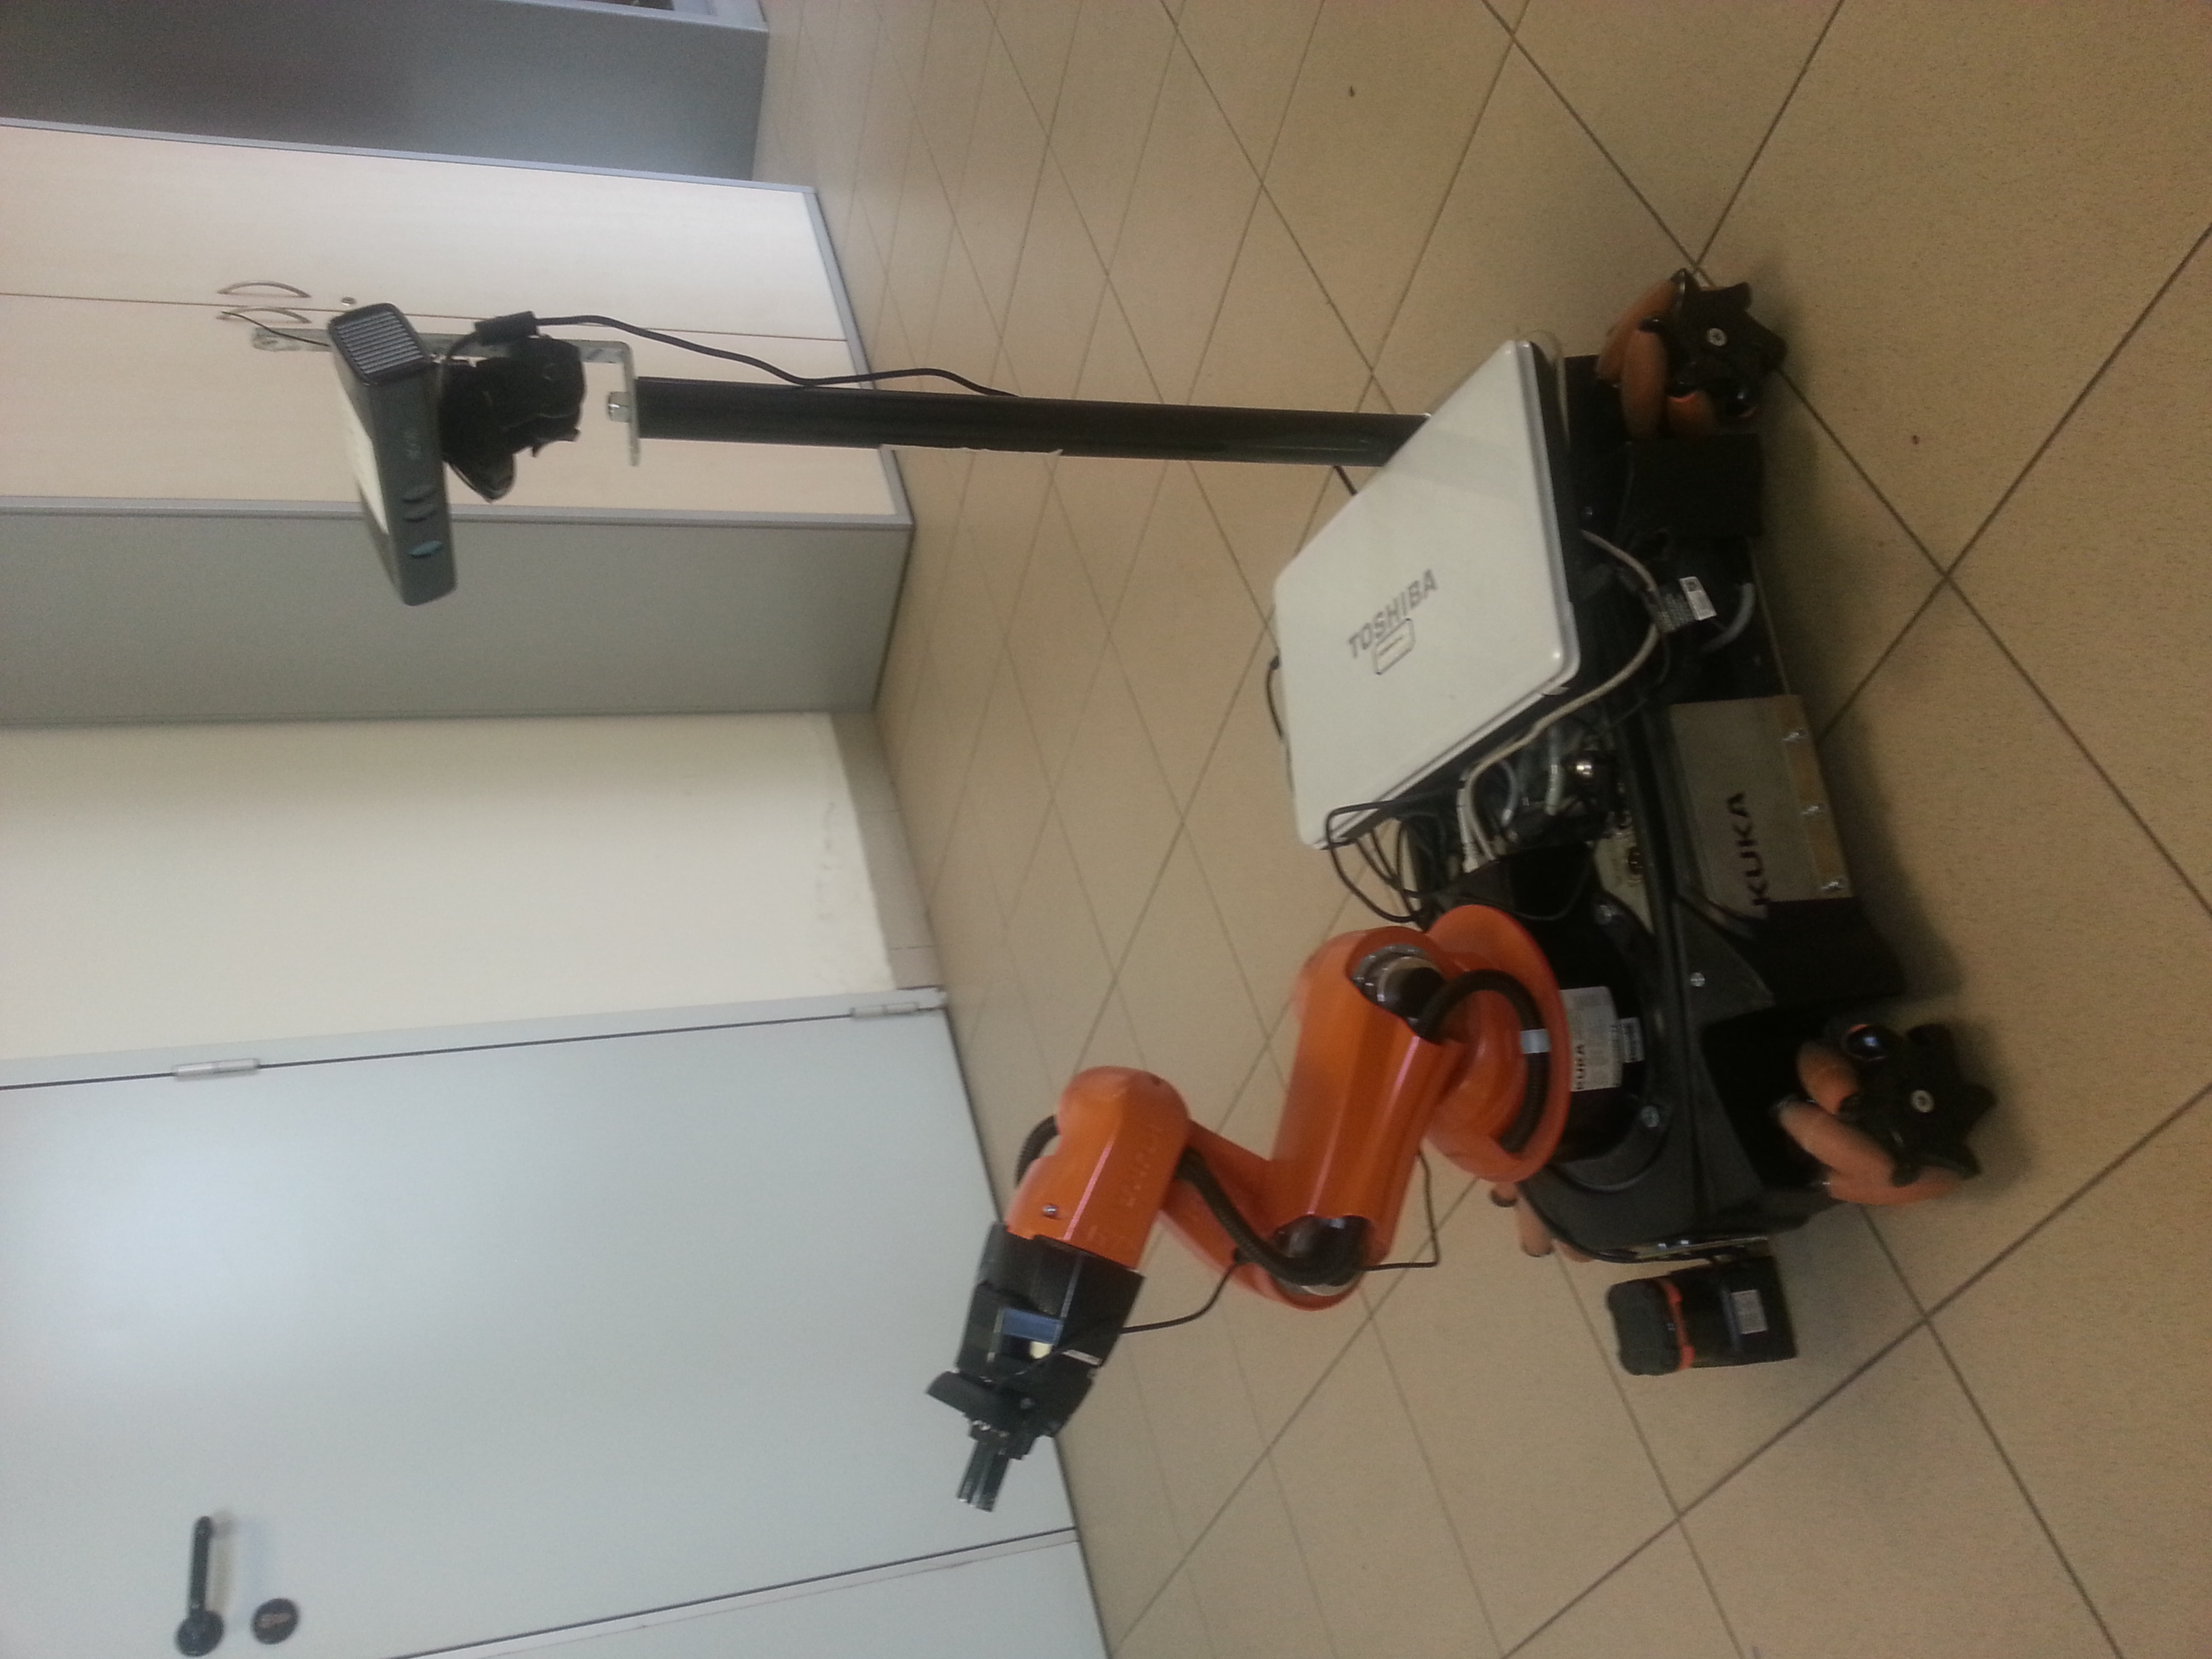
\includegraphics[angle=270,width=0.8\linewidth]{images/test_img.png}
\end{center}
\caption{The ART@Work robot: the laptop is used for computationally expensive tasks (localization, mapping, object recognition, \dots) while the internal standard Intel Atom PC is used for low-level motions controls (platform and arm).}\label{fig:robot}
\end{figure}

\subsubsection{RoCoCo} The laboratory RoCoCo (Cognitive Cooperating Robots) is located at DIAG (Dipartimento di Ingegneria Informatica, Automatica e Gestionale) of Sapienza University of Rome, Italy.
The research developed at RoCoCo laboratory is in the area of Artificial Intelligence and Robotics. RoCoCo has been involved in RoboCup competitions since 1998 in different leagues: Middle-size 1998-2002, Four-legged 2000-2007, Real-rescue-robots 2003-2006, @Home in 2006, Virtual-rescue since 2006 and Stan-dard platform League (Nao Division) since 2008.\\

\subsubsection{IAS-Lab} IAS-Lab stands for Intelligent Autonomous Systems Laboratory and it is one of the 28 laboratories of the Department of Information Engineering of the University of Padua.
The activity at IAS-Lab concerns the study of several fields of Robotics: computer vision, humanoids and wheeled robot programming, virtual simulation, biomechanical model based on human biosignal and wearable robots design for rehabilitation purposes. IAS-Lab has been involved in RoboCup competitions between 1998 and 2006 in Middle-size and humanoids leagues.\\

\subsection{Competence of Team Members}

\subsubsection*{Marco Imperoli}
Imperoli is attending the Master degree in Artificial Intelligence and Robotics Engineering at the Sapienza University of Rome.
\subsubsection*{Michele Marostica}
Marostica received his Master Degree from University of Padua in 2013. The thesis involved the investigation of a novel visual-inertial approach to the loop closure problem for humanoids navigation. His main field of robotics are SLAM and computer vision.
% Since November 2013 he will work for one year on the \textit{DODICH}\footnote{website at http://www.ethics.it/dodich} project, thanks to a research fellowship granted by Regione Veneto.
% The aim is to develop a robot that is able to perform navigation and simple operations in vineyards.
\subsubsection*{Nicolò Boscolo}
Boscolo received his Master Degree from University of Padua in 2012. 
% During the Master Thesis, he started cooperating with IAS-Lab (Intelligent and Autonomous System Laboratory) of the University of Padua where he developed a multi-robot collision aware system that led to a publication presented at IAS-12 conference. 
In 2012 he started working at IT+Robotics, here he is involved in the development of projects about industrial robotics: from motion planning to the simulation and system prototyping. 
% He is also a member of a European project about automated quality control.
Since January 2014 he will enter into the Doctoral School of the Dept. of Information Engineering and the University of Padua as a PhD candidate on Robotics.
\subsubsection*{Roberto Capobianco}
Capobianco received the Master Degree in Artificial Intelligence and Robotics from the Department of Computer, 
Control and Management Engineering (DIAG) of Sapienza University of Rome. 
% During his Master's Thesis he worked in the field of Semantic Mapping, publishing a conference paper and a workshop paper on the same topic. After graduating at M.Sc. (110/110 cum laude) and successfully completing the Excellence Program, 
After graduating, he started his Ph.D. program on November 01, 2013 at the same University. His areas of interest include robot learning, industrial and mobile robotics, and computer vision.
\subsubsection*{Jacopo Serafin}
Serafin obtained the Master of Science in Artificial Intelligence and Robotics from the Department of Computer, Control and Management Engineering (DIAG) of Sapienza University of Rome in March 2013. 
% Right after graduating at M.Sc.(110/110 cum laude) he has been involved in the ROVINA European project where he actually work as responsible for the 3D mapping. 
In November 2013 he started the Ph.D. program in engineering in computer science. His areas of interest include mobile robotics, computer vision, acquisition of 3D models / maps, SLAM and least-squares estimation problems.
\subsubsection*{Alberto Pretto}
Pretto is Assistant Professor at at Sapienza University of Rome since October 2013. 
He received his Ph.D. degree in October 2009 from the University of Padua, where he worked as a postdoctoral researcher at the Intelligent Autonomous Systems Lab (Department of Information Engineering). 
% Between 2011 and 2012 he spent a 9 months visiting research fellowships at the UCLA VisionLab, Los Angeles (USA).
% In 2004 and 2005, he has been working as software engineer at Padua Ricerca Scpa. 
In 2005, he was one of the funders of IT+Robotics Srl, a spin-off company of the University of Padua working on robotics and machine vision. 
Alberto Pretto's main research activities include vision-based 3D reconstruction, visual-inertial navigation, and object recognition.
\subsubsection*{Daniele Nardi}
Nardi is Full Professor at DIS, where he was employed since 1986. His current research interests are in the field of artificial intelligence and cognitive robotics. He is Trustee of RoboCup and currently the president of the RobotCup Federation.  From 2005-2008, he also served as the co-chair of IEEE Technical Committee of International Workshop on Safety, Security and Rescue Robotics.  He is active in the context of autonomous rescue robots and successfully coordinated a team participating on several editions of RoboCup Rescue since the year 2002.  
Nardi received the ``IJCAI-91 Publisher's Prize'' and the prize ``Intelligenza Artificiale 1993'' from the Associazione Italiana per l'Intelligenza Artificiale (AI*IA).
\subsubsection*{Enrico Pagello}
Pagello received his “Laurea” Degree in Electronic Engineering from the Univ. of Padua, Italy, in 1972. From 1976 to 1983, he was a Researcher at the Inst. of Biomedical Eng. of the Nat. Research Council of Italy, where he is now a part-time Senior Associated Researcher. Since 1983 he has joined the School of Engineering, Univ. of Padua, where he is a Professor of Computer Science. 
During 1977-78, he was a Visiting Scholar at the Lab. of A.I. of Stanford Univ. Since 1994, he has regularly visited the Dept. of Precision Engineering, Univ. of Tokyo. In 2005 he was an Invited Professor at Keio Univ. He spent six months in Japan as a Senior JSPS Fellow, both in 2004 and 2008. His current research interests include the application of A.I. to Robotics with particular regard to the Multi-robot Systems, Humanoids and Robot Programming Languages domains. 
% He was a General Chair of the Sixth IAS Conference in July 2000, of RoboCup-2003, and of SIMPAR-2008 Conference. He was a member of the Ed. Board of the IEEE/TRA, and he is currently a member of the Ed. Board of Int. J. of Rob. and Autonomous Sys. He was a President of the Int. Society for Intelligent Autonomous Systems from 2004 to 2012. In 2009 he has been elected Fellow of the School of Engineering of the University of Tokyo.

\subsection{RoCKIn Events participations}
Serafin and Capobianco participated at the RoCKIn Camp 2014 with the ``SPQR Team'', Marostica and Boscolo participated at the RoCKIn Camp 2014 with the ``IAS-Lab Team''. ``SPQR'' and ``IAS-Lab'' teams won in ex-aequo the ``Best Practical in Perception'' award.

\section{Robot Description}

\subsection{Hardware Configuration}

The ART@Work robot (Fig.~\ref{fig:robot}) is a KUKA youBot with the following sensor suite:

\begin{itemize}
 \item A frontal Hokuyo laser scanner, to be used for navigation and obstacles avoidance tasks
 \item A Kinect RGB-D sensor: the area viewed by the kinect includes the working area of the arm, in order to perform object manipulation tasks without robot motions
 \item An on-board laptop (other than the internal standard Intel Atom PC) running Linux Ubuntu 12.04, to be used to execute the perception and planning tasks (e.g., navigation and object recognition)
 \item A color USB camera on the 5th joint of the manipulator for accurate object localization
\end{itemize}
 
\subsection{Software Configuration}

The ART@Work software infrastructure is based on the ROS Groovy middleware running on Ubuntu 12.04, nevertheless most of the developed software tools are stand-alone, middleware-agnostic: packages are integrated within ROS by means of suitable wrappers.\\
The navigation stack is based on particle filter based localization and mapping algorithms, provided by the ROS AMCL and GMapping packages, the latter implemented by one member of the laboratory RoCoCo. The decision making and planning stacks are based on a finite state machine implemented with the ROS Actionlib and MoveBase packages, while manipulation tasks are performed using the MoveIT! ROS package.
3D environment reconstruction is obtained using an effective and efficient registration method called PWN (Point With Normals) (Sec.~\ref{sec:pwn}). 
PWN takes advantage of the 3D structure in determining the data association between two clouds by considering each point along with the statistics of the local surface and of the measurement noise. A novel formulation has been proposed to address the computation of the alignment that takes advantage of point position and surface normals.\\

Object recognition and localization is obtained using reliable algorithms that exploit both vision features and depth information (Sec.~\ref{sec:object_rec}). This module includes a pipeline of processing blocks (Fig.~\ref{fig:pipeline}): the pipeline includes processing blocks for sub-sampling, clustering, noise reduction, and 2D and 3D features detection and descriptors. The model matching step is performed associating the extracted features with features pre-computed from a rigid template (e.g., the CAD model) of the object, sample consensus methods is used to reduce outliers. The result is a set of object candidates, that is refined using an iterative optimization strategy. 

\begin{figure*}[t!]
\begin{center}
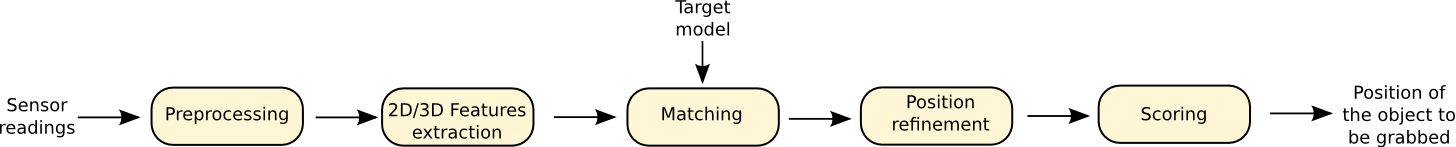
\includegraphics[angle=0,width=\linewidth]{images/pipeline.png}
\end{center}
\caption{The ART@Work object recognition and localization pipeline.}\label{fig:pipeline}
\end{figure*}

Both the mapping and the object recognition modules have been internally implemented by the team members.
Moreover, the ART@Work software includes a semantic mapping system in order to obtain a rich and meaningful representation of the environment (see Sec.~\ref{sec:semantic_map}).\\

Currently, the ART@Work robot is able to:

\begin{itemize}
 \item Localize itself and safely navigate toward a selected target area
 \item Build detailed 3D maps of the surrounding environment
 \item Detect QR code-like markers using vision (using the datamatrix\_finder ROS package, modified by the ART@Work team members)
 \item Recognize and localize objects using RGB-D sensors, using the techniques proposed in \cite{antonelloVISIGRAPP2014} and \cite{prettoCASE2013}
 \item Perform simple visual servoing and manipulation tasks (e.g., pick and place task, ``cutting a string'' task, \dots)
 \item Capture and understand simple audio signals from the environment
\end{itemize}

 
\section{Research areas and Contributions}\label{sec:research}

Several research areas are involved in the ART@Work team development, and some novel contributions have been proposed. Among others, PWN (Sec.~\ref{sec:pwn}), a semantic mapping and learning system (Sec.~\ref{sec:semantic_map}) and a flexible 3D localization system for industrial bin-picking (Sec.~\ref{sec:object_rec}).

\subsubsection{Point Cloud Registration}\label{sec:pwn}

\begin{figure}[t!]
\begin{center}
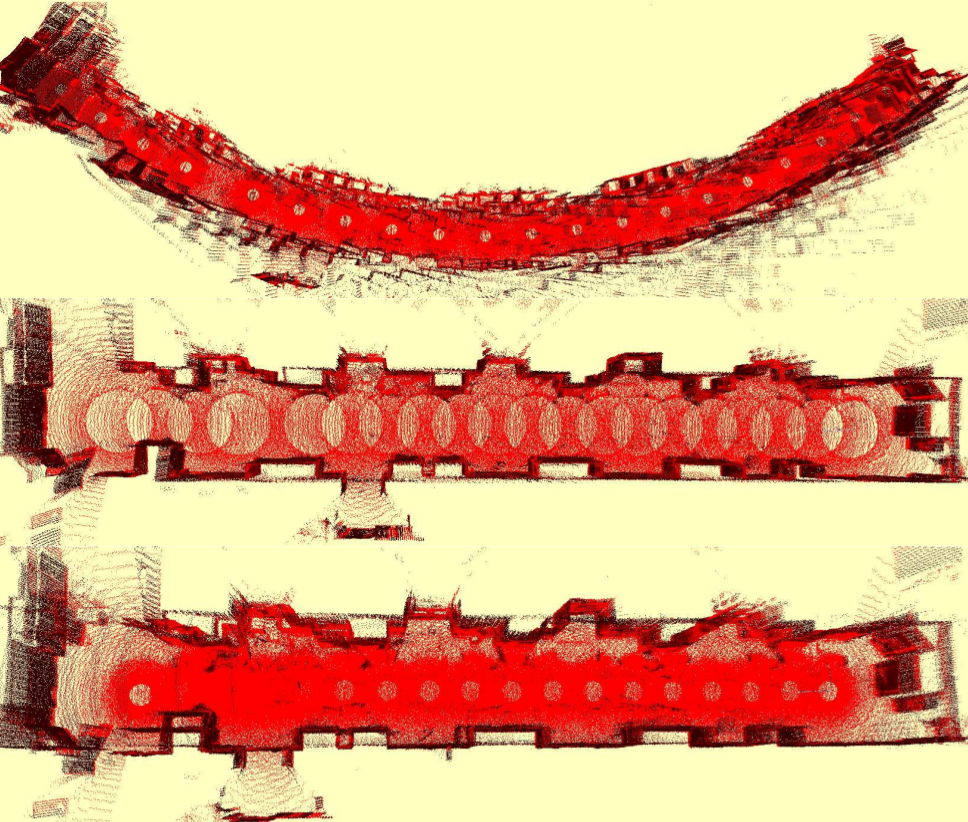
\includegraphics[angle=0,width=\linewidth]{images/pwn.png}
\end{center}
\caption{A 3D scene reconstructed from 3D scans. Top: initial guess. Middle: reconstruction with PWN, done in about 2.16s. Bottom: reconstruction with Generalized ICP, done in about 13.35s. The corridor looks shortened due to a missing frame that caused GICP to fail.}\label{fig:pwn}
\end{figure}

3D models of objects and environments are of utmost importance for a wide range of robotic applications such as navigation, object recognition, manipulation and many others. Hence, being able to acquire these models with the on-board sensors is a necessary precondition for a truly autonomous mobile robot. 3D data can be represented in different ways, one of them is using point clouds. In the past years many point cloud registration algorithms were developed, these algorithms are procedures used to compute the translation and rotation that maximize the overlap between two point clouds. Point cloud registration is a fundamental building block for a lot of robotics applications like odometry reconstruction, SLAM, navigation and 3D object scanning. During his M.Sc. thesis, Jacopo Serafin developed a new point cloud registration approach (Fig.~\ref{fig:pwn}). He proposed a novel formulation to address the computation of the alignment that takes advantage of point position and surface normals. Additionally, he presented a fast method to merge registered point clouds while refining the point positions and reducing the number of points. This new approach has been named Point With Normal aligner (PWN in short).   

\subsubsection{Semantic Mapping and Learning}\label{sec:semantic_map}
In order to properly act in a complex way and execute difficult tasks, robotics systems need a deep knowledge of the environments and the objects in it. Knowledge representation in robotics, however, is a challenging problem, since not only the chosen abstraction may affect the performance of the robot, but also different kinds of knowledge, depending on the context, may be needed in order to implement complex behaviors. In the case of robots that operate in a physical environment, it is required to “close the loop” with perception, thus defining the relationship between numeric and symbolic representation. During his Master Thesis, Roberto Capobianco worked on a system that incrementally builds a rich representation of the environment, exploiting human-robot interaction in order to perform a collaborative lifelong learning task and to solve ambiguities and possible conflicts in the acquired knowledge \cite{bastianelli2013line}\cite{bastianelliBCGIN13}. Such an interactive approach will be extended to different learning tasks in order to improve the current capabilities of the robots.

\subsubsection{Object Recognition and Localization}\label{sec:object_rec}
A reliable and accurate object recognition system is an essential prerequisite to successfully compete in the RoCKIn competitions. The ART@Work team members presented a robust and flexible vision system for 3D localization of objects for industrial robots \cite{prettoCASE2013} (Fig.~\ref{fig:obj_rec}). This system can estimate the 6 degrees of freedom (DoF) pose of planar objects from a single 2D image.
The localization software is based on a two step strategy: i) a candidates selection step based on a well-engineered voting scheme ii) a refinement and best match selection step based on a robust iterative optimize-and-score procedure. During this second step, a novel strategy called search-in-the-stack has employed, that avoids the optimization from
being stuck on local minima (representing false positives) created when objects are almost regularly stacked.

\subsubsection{Obstacles Avoidance and Manipulation}\label{sec:manipulation}
In order to obtain a reliable robot navigation, ART@Work team members implemented an efficient obstacles avoidance system for mobile robots equipped with range finder sensors, based on the online computation of local artificial potential fields. \newline In the field of manipulation, an effective framework for handling tasks priority of redundant manipulators has been studied and developed.
\begin{figure}[t!]
\begin{center}
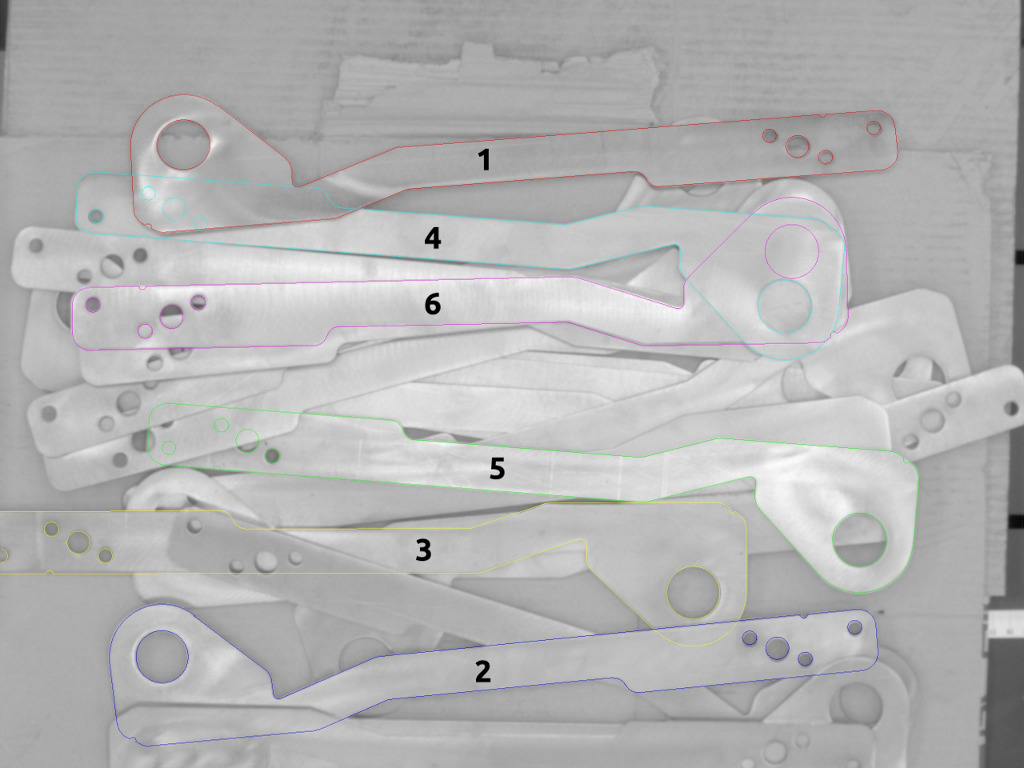
\includegraphics[angle=0,width=\linewidth]{images/result_number01_small.jpg}
\end{center}
\caption{Final results of the proposed localization system.}\label{fig:obj_rec}
\end{figure}

\section{Reusability and Relevance to Industrial Robotics}

\begin{itemize}
 \item PWN (Sec.~\ref{sec:pwn}) became a basic block for a novel traversability analysis algorithm described by Bogoslavskyi et al. in~\cite{bogoslavskyi-ECMR-13}.
 \item The proposed object recognition and localization systems (Sec.~\ref{sec:object_rec}) is currently installed in seven real world industrial plants \footnote{E.g., https://www.youtube.com/watch?v=jqhuEjnDdfI}, with different setups, working with hundreds of different models and successfully guiding the manipulators to pick several hundreds of thousands of pieces per year. 
 \item The proposed task priority manager (Sec.~\ref{sec:manipulation}) is currently implemented inside a real 3D industrial simulator for the off-line programming of workcells and machines with several axis.  \footnote{http://www.it-robotics.it/products/3d-simulation/workcellsimulator/?lang=en}
\end{itemize}

\bibliographystyle{IEEEtran}
\bibliography{bibliography} 

% that's all folks
\end{document}


